% =============================================================================
% Crossbar Switch Chapter – Introduction / Concept
% Copy this into your Overleaf project.
% Required packages (add to your preamble if not already present):
%   \usepackage{tikz}
%   \usepackage{amsmath}
% =============================================================================

\section{Crossbar Switch}
\label{sec:crossbar}

\subsection{Concept and Operating Principle}
\label{subsec:crossbar_concept}

A crossbar switch is one of the most fundamental building blocks in network switch design.
Its purpose is to establish a configurable connection between any input port and any output port, 
allowing data to be routed from its source to its intended destination.
In its most general form, an $N \times N$ crossbar consists of a grid of $N^2$ crosspoints, 
where the $N$ horizontal input lines intersect with the $N$ vertical output lines.
Each crosspoint acts as a programmable switch that can be opened or closed: 
when a crosspoint at position $(i,\,j)$ is closed, input~$i$ is connected to output~$j$ 
and data flows through.
Figure~\ref{fig:classic_crossbar} illustrates this topology for a $4 \times 4$ configuration.

\begin{figure}[htbp]
    \centering
    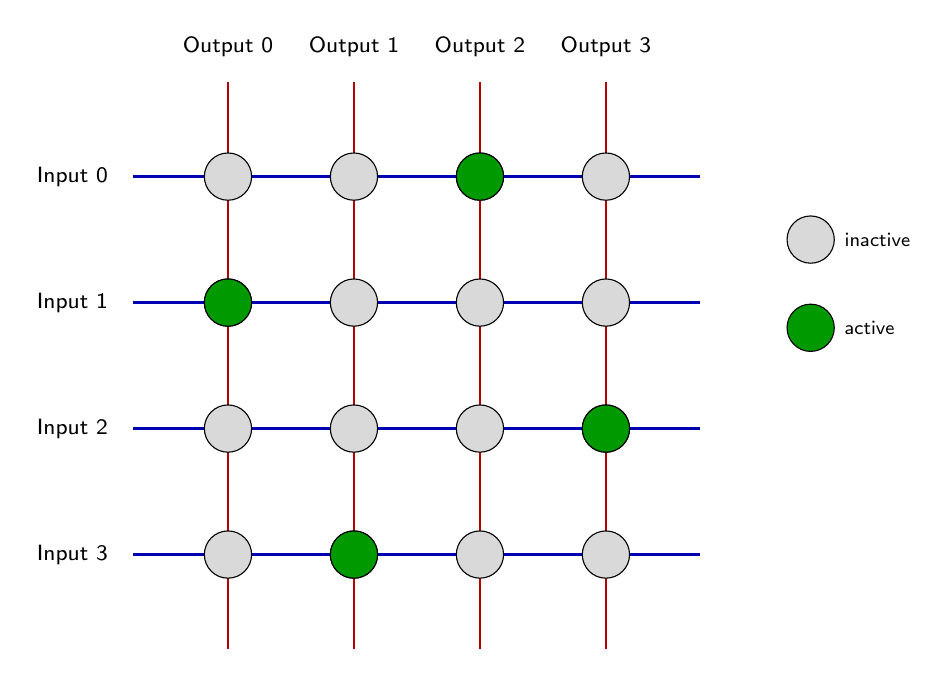
\begin{tikzpicture}[
        scale=1.0,
        crosspoint/.style={circle, draw, fill=black!15, minimum size=6mm, inner sep=0pt},
        crosspoint_active/.style={circle, draw, fill=green!60!black, minimum size=6mm, inner sep=0pt},
        port_label/.style={font=\footnotesize\sffamily},
    ]
    
    % Grid dimensions
    \def\N{4}
    \def\spacing{1.6}
    
    % Draw horizontal lines (inputs)
    \foreach \i in {0,...,3} {
        \draw[thick, blue!70!black] (-1.2, -\i*\spacing) -- (\N*\spacing - \spacing + 1.2, -\i*\spacing);
        \node[port_label, anchor=east] at (-1.4, -\i*\spacing) {Input \i};
    }
    
   \foreach \j in {0,...,3} {
        \draw[thick, red!70!black] (\j*\spacing, 1.2) -- (\j*\spacing, -3*\spacing - 1.2);
        \node[port_label, anchor=south] at (\j*\spacing, 1.4) {Output \j};
    }
    
    % Draw crosspoints (inactive)
    \foreach \i in {0,...,3} {
        \foreach \j in {0,...,3} {
            \node[crosspoint] at (\j*\spacing, -\i*\spacing) {};
        }
    }
    
    % Highlight active connections: 
    %   Input 0 -> Output 2,  Input 1 -> Output 0,  Input 2 -> Output 3,  Input 3 -> Output 1
    \node[crosspoint_active] at (2*\spacing, -0*\spacing) {};  % (0,2)
    \node[crosspoint_active] at (0*\spacing, -1*\spacing) {};  % (1,0)
    \node[crosspoint_active] at (3*\spacing, -2*\spacing) {};  % (2,3)
    \node[crosspoint_active] at (1*\spacing, -3*\spacing) {};  % (3,1)
    
    % Legend
    \node[crosspoint, label={[font=\scriptsize\sffamily]right: inactive}] at (\N*\spacing + 1.0, -0.5*\spacing) {};
    \node[crosspoint_active, label={[font=\scriptsize\sffamily]right: active}] at (\N*\spacing + 1.0, -1.2*\spacing) {};
    
    \end{tikzpicture}
    \caption{Classic $4 \times 4$ crossbar switch topology. Each intersection represents a 
    programmable crosspoint. Green (active) crosspoints indicate the currently established 
    connections: Input~0$\to$Output~2, Input~1$\to$Output~0, Input~2$\to$Output~3, 
    and Input~3$\to$Output~1.}
    \label{fig:classic_crossbar}
\end{figure}

A key property of the crossbar is its non-blocking nature: as long as no two inputs attempt to 
reach the same output simultaneously, all $N$ connections can be active in parallel without 
interference. However, when multiple input ports have data destined for the same output port, 
a conflict --- known as \emph{output contention} --- arises, and only one of the competing inputs 
can be served at any given time. Resolving these conflicts is the task of a 
\emph{scheduling algorithm}, which determines the crossbar configuration for each time slot.

In traditional input-queued (IQ) switch architectures, this scheduling problem is non-trivial. 
Algorithms such as iSLIP perform iterative matching between inputs and outputs over 
multiple rounds within a single clock cycle, which limits the achievable operating frequency 
--- particularly on FPGAs, where deep combinational logic paths directly reduce the maximum 
clock rate. The complexity grows further with the number of ports, as the scheduler must 
evaluate all possible input--output pairings.

The design presented in this work avoids this scheduling bottleneck entirely through the use 
of Virtual Output Queues (VOQs), which pre-sort incoming frames by their destination port 
\emph{before} they reach the crossbar. As a result, the crossbar itself can be implemented as a 
simple set of multiplexers rather than a dynamically scheduled switching matrix. This 
architectural simplification and its FPGA implementation are discussed in the following 
subsection.